Figure \ref{fig:siso-ff-snr} and \ref{fig:siso-fs-snr} contrast the performance of the modulated waveform, ideal superposed waveform and its lower bound for $N = 16$ and ${\text{SNR}} = 10,20,30,40$ dB under the FF and FS channel response in Figure \ref{fig:siso-channels}.

\begin{figure}[ht]
  \centering
  \subfigure[FF: ${\text{SNR}} = 10$ dB]{
    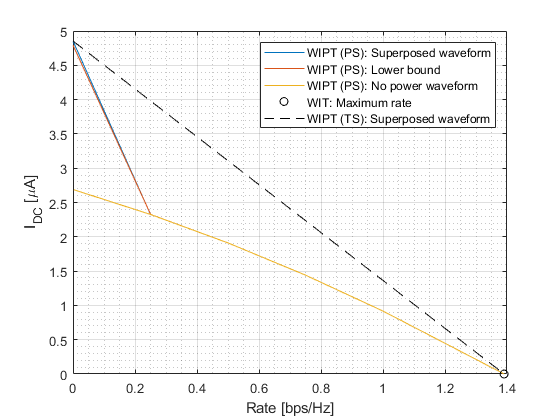
\includegraphics[width=0.48\textwidth]{siso_re_ff_snr_10dB}\label{fig:snr-ff-10db}}
  \subfigure[FF: ${\text{SNR}} = 20$ dB]{
    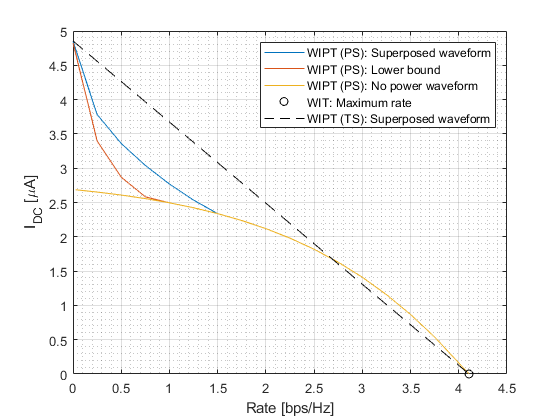
\includegraphics[width=0.48\textwidth]{siso_re_ff_snr_20dB}\label{fig:snr-ff-20db}}
  \quad
  \subfigure[FF: ${\text{SNR}} = 30$ dB]{
    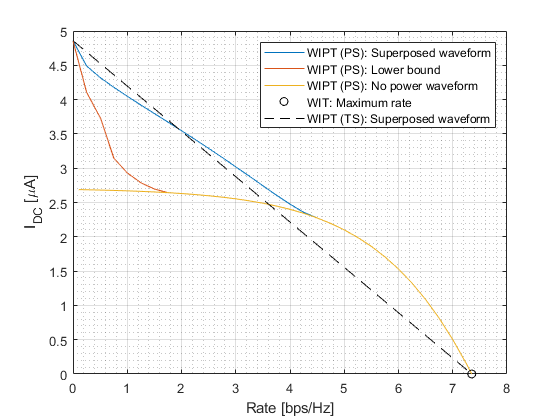
\includegraphics[width=0.48\textwidth]{siso_re_ff_snr_30dB}\label{fig:snr-ff-30db}}
  \subfigure[FF: ${\text{SNR}} = 40$ dB]{
    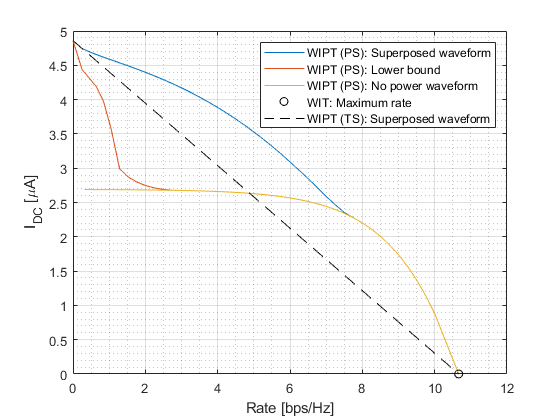
\includegraphics[width=0.48\textwidth]{siso_re_ff_snr_40dB}\label{fig:snr-ff-40db}}
  \caption{R-E region vs SNR for FF channel}\label{fig:siso-ff-snr}
\end{figure}

\begin{figure}[ht]
  \centering
  \subfigure[FS: ${\text{SNR}} = 10$ dB]{
    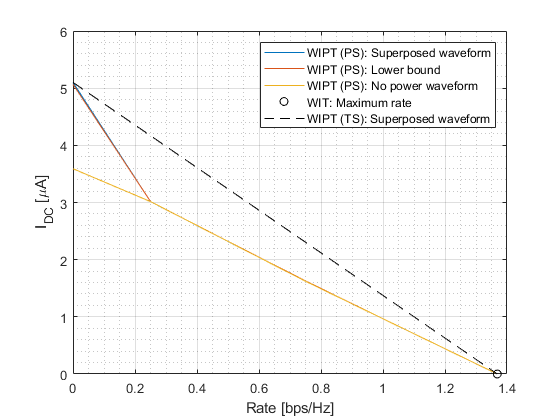
\includegraphics[width=0.48\textwidth]{siso_re_fs_snr_10dB}\label{fig:snr-fs-10db}}
  \subfigure[FS: ${\text{SNR}} = 20$ dB]{
    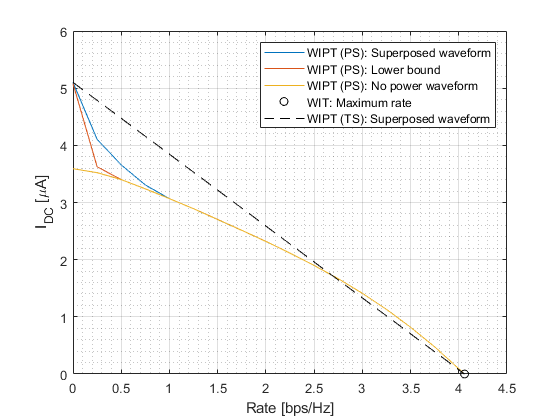
\includegraphics[width=0.48\textwidth]{siso_re_fs_snr_20dB}\label{fig:snr-fs-20db}}
  \quad
  \subfigure[FS: ${\text{SNR}} = 30$ dB]{
    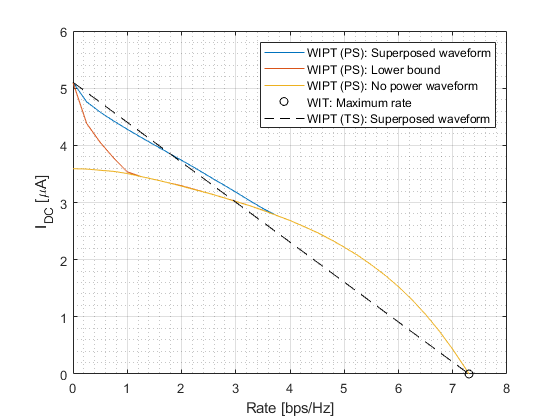
\includegraphics[width=0.48\textwidth]{siso_re_fs_snr_30dB}\label{fig:snr-fs-30db}}
  \subfigure[FS: ${\text{SNR}} = 40$ dB]{
    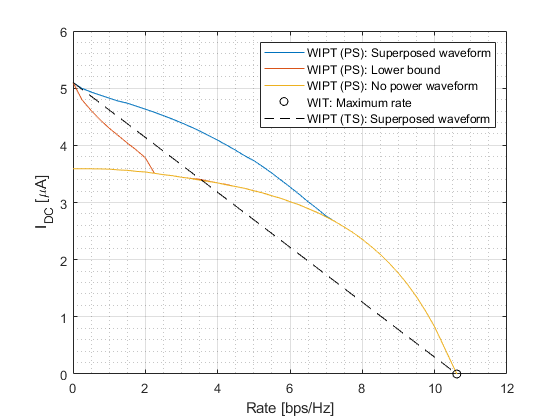
\includegraphics[width=0.48\textwidth]{siso_re_fs_snr_40dB}\label{fig:snr-fs-40db}}
  \caption{R-E region vs SNR for FS channel}\label{fig:siso-fs-snr}
\end{figure}

Compared with the modulated signal, the R-E region of the superposed signal is enlarged for both cases with the contribution of the multisine waveform. This phenomenon is especially obvious in the low-rate region where the multisine dominates the transmission. It results from the fact that the nonlinear rectifier favors the deterministic multisine with high PAPR. On the contrary, there are some randomness involved in the modulated waveform that produces fluctuations to the rectifier and leads to some power loss \cite{Clerckx2018}. This phenomenon is in sharp contrast to the argument in \cite{Xu2014a} that both waveforms are equally suitable for WPT, which is based on the conventional linear harvester model. As shown in Figure \ref{fig:siso-ff-snr} and \ref{fig:siso-fs-snr}, even with the assumption that the deterministic power waveform creates some interference to the information waveform, the rate loss is compensated by the power gain such that the superposed waveform strictly outperforms the modulated waveform.

Another observation is that the gap of R-E region between the ideal superposed waveform and its lower bound widens as SNR increases. This is as expected because the rate is dominated by noise at low SNR and by interference at high SNR. For ${\text{SNR}} = 10$ dB, the interference is far lower than noise even if a large amount of power is allocated to the multisine component, and the curves almost overlap with each other. On the other hand, for a higher SNR as 30 dB, the rate loss by interference increases while the energy benefit of power waveform remains unchanged. To obtain the optimal R-E tradeoff, the transmitter tends to allocate less power to the multisine so that the difference in harvested current increases for a fixed rate. Therefore, the rate boost of deterministic power waveform grows as SNR increases.

It also demonstrates that for the superposed waveform with a sufficiently large $N$, TS is preferred at low SNR and PS is favored at high SNR, while a combination of TS and PS is generally optimal for medium SNR. On the other hand, the R-E region is strictly convex for the modulated waveform-only transmission due to its inefficiency to boost the harvested energy. It suggests that PS always outperforms TS for no power waveform no matter the SNR. Moreover, the corresponding R-E curve is approximately straight at low SNR but with large curvature at high SNR. The reason is that for a low SNR, the water-filling strategy concentrates the power to the best subband to maximize the rate, and the region boundary is obtained by varying $\rho $ only. In comparison, more subbands are utilized in the transmission as SNR increases. Therefore, only a small portion of power is required to achieve a decent rate such that the output DC current can be maintained at a high level.

A comparison between the results over FF and FS channels emphasizes the benefit of frequency selectivity on the harvested current. The gain is more significant for modulated waveform (around \SI{1}{\uA}) than superposed waveform (around \SI{0.25}{\uA}). One possible reason is that the power are concentrated in few subbands such that the number of terms in \ref{eqn:power_waveform_fourth_order} and \ref{eqn:information_waveform_fourth_order} are comparable. In such cases, the impact of channel amplitude on each monomial is more significant on the information waveform and contributes to a larger gain in the harvested current.

